In range query with $K$D-tree, we traverse the whole tree with a pruning strategy. Similarly, to perform $K$NN query with $K$D-tree, we also need to traverse the whole tree with a pruning strategy. We first present how to perform the nearest neighbour query (i.e. a $K$NN query with $K=1$), and then extend it into general $K$NN query.

\begin{figure}[!htb]
     \centering
     \begin{subfigure}[b]{0.58\textwidth}
         \centering
         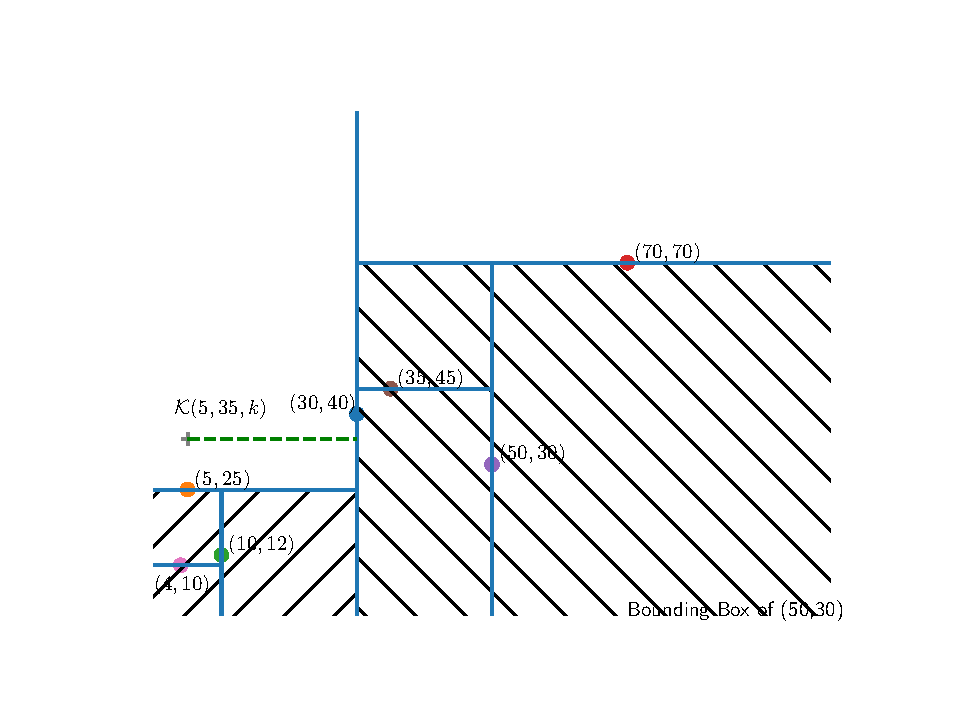
\includegraphics[width=\textwidth]{graphs/implementation/queries/knn_query_kdtree}
         \caption{The $2$D space and the partition of $K$D-tree}
     \end{subfigure}
     \hfill
     \begin{subfigure}[b]{0.40\textwidth}
         \centering
         \begin{tikzpicture}
\tikzstyle{bplus}=[rectangle split, rectangle split horizontal,rectangle split ignore empty parts,draw]
\tikzstyle{every node}=[bplus]
\tikzstyle{level 1}=[sibling distance=30mm]
\tikzstyle{level 2}=[sibling distance=15mm]
\node {(30,40)} [->]
  child {node {(5,25)}
    child {node {(10,12)}
    	child {node {(4,10)}}
    	child[missing]{}
    }
    child[missing]{}    
  } 
  child {node {(70,70)}
    child {node {(50,30)}
    	child {node {(35,45)}}
    	child[missing]{}
    }
    child[missing]{}
  }
;\end{tikzpicture}
         \caption{The tree structure of the $K$D-tree}
     \end{subfigure}
        \caption{An example of $K$NN Query with $K$D-Tree}
        \label{fig:kdtree-knnquery}
\end{figure}

\noindent
\textbf{Nearest Neighbours}

During the query for the nearest neighbour, we use two global variables \texttt{best} and \texttt{best\_dist} to store the nearest node and the nearest distance. During the traversing of the tree, we update the best points and the best distance if we find a closer node to the query point.

Similar to the pruning strategy in the range query with $K$D-tree, we can calculate the distance between the query point to a bounding box of a node. If the query point is inside the bounding box, then the distance will be $0$. If the current shortest distance is larger than or equal to the distance between the query point and the bounding box, then there will not be any points that are closer to the query point than the current closes point. Therefore, we can avoid searching the subtree that will not contain any closer points.

With the pruning strategy, we traverse the tree in an order that maximises the change for pruning. We always start with the subtree that are closer to the query point. In other words, we search the subtree that would contain the query point if we want to insert the query point below the root of a subtree.

\begin{mscexample}
	For example, we demonstrate an example $K$NN query $\mathcal{K}(5, 35, k)$ whose query point is $(5, 35)$ in Fig. \ref{fig:kdtree-knnquery}. We perform the nearest neighbour search in the following order.
	
	\begin{enumerate}
		\item First we start with the root node, which is $(30,40)$. The bounding box of the root node is the whole space, and we cannot apply the pruning strategy. If we want to insert the query point $(5, 35)$ into the subtree rooted at the root node, we will insert it into the left subtree by comparing the $x$-coordinate. Hence, we go to the left subtree in the next step. At the root level, the best distance is $\sqrt{(30-5)^2+(40-35)^2}=25.5$ and the closet point is $(30,40)$.
		\item Then we traverse to the left subtree and calculate the distance. The bounding box of this node is $\boldsymbol{l}=(0,0)$ and $\boldsymbol{u}=(30,100)$. The distance between the query point and the bounding box will be $0$ as it contains the query point. Hence we cannot apply the pruning strategy. The distance is $10$ and it is smaller than the old distance. Hence at this level, the best distance is $10$ and the closest point is $(5,25)$. Then if we want to insert the query point into the subtree under $(5,25)$, we will compare the $y$-coordinate and then we need to first traverse the right subtree.
		\item As there is no right subtree, we still go to the left subtree. The bounding box of this node is $\boldsymbol{l}=(0,0), \boldsymbol{u}=(30,25)$ and the distance between the bounding box and the query point is $10$. The distance is the same with the best distance so far. Therefore we apply the pruning strategy and do not need to traverse the subtree.
		\item Similarly, for the right subtree of the root node, $(70,70)$ whose bounding box is $\boldsymbol{l}=(30,0), \boldsymbol{u}=(100,70)$, the distance between the query point and the bounding box is $\sqrt{(30-5)^2+(40-35)^2}=25.5$, which is larger than the current best distance. Therefore we apply the pruning strategy and do not traverse the right subtree of the root.
	\end{enumerate}
\end{mscexample}

\noindent
\textbf{$K$-Nearest Neighbours}

For general $K$NN query, we follow the same traversal and pruning strategy. The only difference is that we use a max heap of size $k$ to store the best $K$ distance we have.

A max heap is a special binary tree that satisfies a property: if \texttt{P} is a parent node of \texttt{C}, then the data in \texttt{P} is greater than or equal to the data in \texttt{C}. We store the max heap as a binary tree and use a function \texttt{heapify} to make it a max heap.

Then we follow the steps below to construct and fill the max heap:

\begin{enumerate}
	\item First we construct an empty binary tree. 
	\item We traverse the $K$D-tree with the pruning strategy as described in the nearest neighbour query. For each element, we decide if we need to push it into the max heap in the following way:
	\begin{itemize}
		\item For the first $K$ elements, they will be added to the binary tree no matter how close it is to the query point. We call the \texttt{heapify} function to ensure the resulting binary tree is a max heap.
		\item After the $K$th element, we compare the distance between the element and the query point with the root of the binary tree. Since we have used \texttt{heapify} and the root is the largest distance so far.
		\begin{itemize}
			\item If the distance is smaller than the root, then we make it root and call \texttt{heapify}.
			\item Otherwise, we ignore it.
		\end{itemize}
	\end{itemize}
	\item Finally the max heap has $K$ smallest elements and the root of the heap is the $K$th smallest element.
\end{enumerate}

Formally, we use the algorithms as illustrated in Algo. \ref{algo:kd-tree-knn} to perform $K$NN query with $K$D-tree.

% Please double check this algorithm.

\begin{algorithm}[H]
\SetAlgoLined
\SetKwInOut{Input}{input}
\Input{\texttt{P}: The query point; \texttt{T}: The root node of a subtree to be searched; \texttt{K}: The number of nearest neighbours \texttt{H}: the binary tree that storing the result; \\ \texttt{cd}: Current dimension}
\KwResult{\texttt{H}: The binary tree that storing the result}
	\texttt{DIM = 2}\\
	\uIf{\texttt{T==NULL}} {
		\Return ;
	}
	\uIf{\texttt{H.size()<K}} {
		\texttt{H.insert(T)}\\
		\texttt{H.heapify()}\\
		\Return ;
	}
	\uElseIf{\texttt{dist(P, T.range) > H.root.data}} {
		\Return ;
	}
	\uElse{
		\uIf{\texttt{dist(P, T.data) < H.root.data}} {
			\texttt{N=NewBinaryTreeNode(dist(P, T.data))}\\
			\texttt{N.insert(H)}\\
			\texttt{N.heapify()}\\
			\texttt{H=N}\\
		}
		\uIf{\texttt{P[cd]<T.data[cd]}}{
			\texttt{KNN(P, T.left, K, H, (cd+1)\%DIM)} \\ 
			\texttt{KNN(P, T.right, K, H, (cd+1)\%DIM)}
		}
		\uElse{
			\texttt{KNN(P, T.right, (cd+1)\%DIM, K, H)} \\ 
			\texttt{KNN(P, T.left, (cd+1)\%DIM, K, H)}

		}
	} 
 \caption{$K$D-tree $K$NN Query}
 \label{algo:kd-tree-knn}
\end{algorithm}